\newcommand{\ransomwareTagResultsAucTable}{
    \begin{table}[H]
        \centering
        \begin{tabular}{|p{2,8cm}||p{2,8cm} p{2,8cm} p{2,8cm}|}
            \hline
            Ransomware Tag & ALOHA & Joint Embedding & Proposed Model \\
            \hline
            AUC-ROC & 0.451$\pm$0.039 & 0.448$\pm$0.028 & \textBF{0.503$\pm$0.023} \\
            \hline
        \end{tabular}
        \caption{AUC-ROC (Area Under Curve) of the different models for the \textbf{Ransomware Tag} prediction task. Results were aggregated over \textBF{3} training runs with different weight initializations and minibatch orderings. Best results are shown in \textbf{bold}.} \label{tab:ransomwareTag_auc}
    \end{table}
}

\newcommand{\ransomwareTagResultsAtFprTable}{
    \begin{center}
        \begin{longtable}[c]{|p{3,2cm}||p{1,8cm} p{1,8cm} p{1,8cm} p{1,8cm} p{1,8cm}|}
            \hline
            Ransomware Tag & \multicolumn{5}{c|}{{FPR}} \\
            & $10^{-5}$ & $10^{-4}$ & $10^{-3}$ & $10^{-2}$ & $10^{-1}$ \\
            \hline
            \endfirsthead

            \caption*{\raggedright ...continued from previous page} \\
            \hline
            Ransomware Tag & \multicolumn{5}{c|}{\textbf{FPR}} \\
            & $10^{-5}$ & $10^{-4}$ & $10^{-3}$ & $10^{-2}$ & $10^{-1}$ \\
            \hline
            \endhead

            \caption*{\raggedleft ...continued on next page} \\
            \endfoot

            \caption{Mean and standard deviation results (TPR, Accuracy, Recall, Precision and F1-Score) of the different models for the \textbf{Ransomware Tag} prediction task at different \textbf{FPR}s (\textit{False Positive Rates}). Results were aggregated over \textBF{3} training runs with different weight initializations and minibatch orderings. Best results are shown in \textbf{bold}. Under \textbf{TPR} results are also presented the percentage reduction in mean detection error and in ROC curve standard deviation introduced by the \textit{Proposed Model} with respect to both \textit{ALOHA} model and \textit{Joint Embedding}.} \label{tab:ransomwareTag_results_at_fpr} \\
            \endlastfoot

            \multicolumn{6}{|c|}{\textbf{TPR}} \\
            \hline
            ALOHA & 0.000$\pm$0.000 & 0.000$\pm$0.000 & 0.000$\pm$0.000 & \textBF{0.024$\pm$0.000} & 0.082$\pm$0.038 \\
            Joint Embedding & 0.000$\pm$0.000 & 0.000$\pm$0.000 & 0.004$\pm$0.006 & 0.008$\pm$0.011 & \textBF{0.090$\pm$0.039} \\
            Proposed Model & \textBF{0.004$\pm$0.006} & \textBF{0.004$\pm$0.006} & \textBF{0.008$\pm$0.006} & 0.020$\pm$0.006 & 0.078$\pm$0.020 \\
            \hline
            Error Reduction wrt \newline ALOHA & 0.4\% & 0.4\% & 0.8\% & -0.4\% & -0.4\% \\
            Error Reduction wrt \newline Joint Embedding & 0.4\% & 0.4\% & 0.4\% & 1.2\% & -1.3\% \\
            \hline
            Std Reduction wrt \newline ALOHA & 0.0\% & 0.0\% & 0.0\% & 0.0\% & 47.4\% \\
            Std Reduction wrt \newline Joint Embedding & 0.0\% & 0.0\% & 0.0\% & 45.5\% & 48.7\% \\
            \hline
            \multicolumn{6}{|c|}{\textbf{Accuracy}} \\
            \hline
            ALOHA & \textBF{0.965$\pm$0.000} & \textBF{0.965$\pm$0.000} & \textBF{0.965$\pm$0.000} & 0.957$\pm$0.000 & 0.872$\pm$0.001 \\
            Joint Embedding & \textBF{0.965$\pm$0.000} & \textBF{0.965$\pm$0.000} & \textBF{0.965$\pm$0.000} & \textBF{0.961$\pm$0.001} & \textBF{0.875$\pm$0.003} \\
            Proposed Model & \textBF{0.965$\pm$0.000} & \textBF{0.965$\pm$0.000} & 0.965$\pm$0.001 & 0.959$\pm$0.002 & 0.873$\pm$0.002 \\
            \hline
            \multicolumn{6}{|c|}{\textbf{Recall}} \\
            \hline
            ALOHA & 0.000$\pm$0.000 & 0.000$\pm$0.000 & 0.000$\pm$0.000 & \textBF{0.024$\pm$0.000} & 0.082$\pm$0.038 \\
            Joint Embedding & 0.000$\pm$0.000 & 0.000$\pm$0.000 & 0.004$\pm$0.006 & 0.008$\pm$0.011 & \textBF{0.090$\pm$0.039} \\
            Proposed Model & \textBF{0.004$\pm$0.006} & \textBF{0.004$\pm$0.006} & \textBF{0.008$\pm$0.006} & 0.020$\pm$0.006 & 0.078$\pm$0.020 \\
            \hline
            \multicolumn{6}{|c|}{\textbf{Precision}} \\
            \hline
            ALOHA & \textBF{1.000$\pm$0.000} & \textBF{1.000$\pm$0.000} & 0.000$\pm$0.000 & 0.080$\pm$0.000 & 0.029$\pm$0.013 \\
            Joint Embedding & \textBF{1.000$\pm$0.000} & \textBF{1.000$\pm$0.000} & 0.167$\pm$0.236 & 0.042$\pm$0.059 & \textBF{0.032$\pm$0.012} \\
            Proposed Model & \textBF{1.000$\pm$0.000} & \textBF{1.000$\pm$0.000} & \textBF{0.500$\pm$0.408} & \textBF{0.096$\pm$0.006} & 0.028$\pm$0.007 \\
            \hline
            \multicolumn{6}{|c|}{\textbf{F1 Score}} \\
            \hline
            ALOHA & 0.000$\pm$0.000 & 0.000$\pm$0.000 & 0.000$\pm$0.000 & \textBF{0.036$\pm$0.000} & 0.042$\pm$0.019 \\
            Joint Embedding & 0.000$\pm$0.000 & 0.000$\pm$0.000 & 0.008$\pm$0.011 & 0.013$\pm$0.019 & \textBF{0.047$\pm$0.019} \\
            Proposed Model & \textBF{0.008$\pm$0.011} & \textBF{0.008$\pm$0.011} & \textBF{0.015$\pm$0.011} & 0.032$\pm$0.008 & 0.041$\pm$0.011 \\
            \hline
        \end{longtable}
    \end{center}
}

\newcommand{\ransomwareTagResultsSummaryTable}{
    \begin{table}[H]
        \centering
        \begin{tabular}{|p{3,2cm}||p{1,8cm} p{1,8cm} p{1,8cm} p{1,8cm} p{1,8cm}|}
            \hline
            \multicolumn{6}{|c|}{Ransomware Tag (at FPR $=1\%$)} \\
            \hline
            Model & TPR & Accuracy & Precision & Recall & F1 score \\
            \hline
            ALOHA & \textBF{0.024$\pm$0.000} & 0.957$\pm$0.000 & 0.080$\pm$0.000 & \textBF{0.024$\pm$0.000} & \textBF{0.036$\pm$0.000} \\
            Joint Embedding & 0.008$\pm$0.011 & \textBF{0.961$\pm$0.001} & 0.042$\pm$0.059 & 0.008$\pm$0.011 & 0.013$\pm$0.019 \\
            Proposed Model & 0.020$\pm$0.006 & 0.959$\pm$0.002 & \textBF{0.096$\pm$0.006} & 0.020$\pm$0.006 & 0.032$\pm$0.008 \\
            \hline
        \end{tabular}
        \caption{Summary of the mean and standard deviation results of the different models for the \textbf{Ransomware Tag} prediction task at \textbf{FPR} $=1\%$. Results were aggregated over \textBF{3} training runs with different weight initializations and minibatch orderings. Best results are shown in \textbf{bold}.} \label{tab:ransomwareTag_result_summary}
    \end{table}
}

\newcommand{\ransomwareTagRocAloha}{
    \begin{figure}[H]
        \vspace*{-0.5cm}
        \centering
        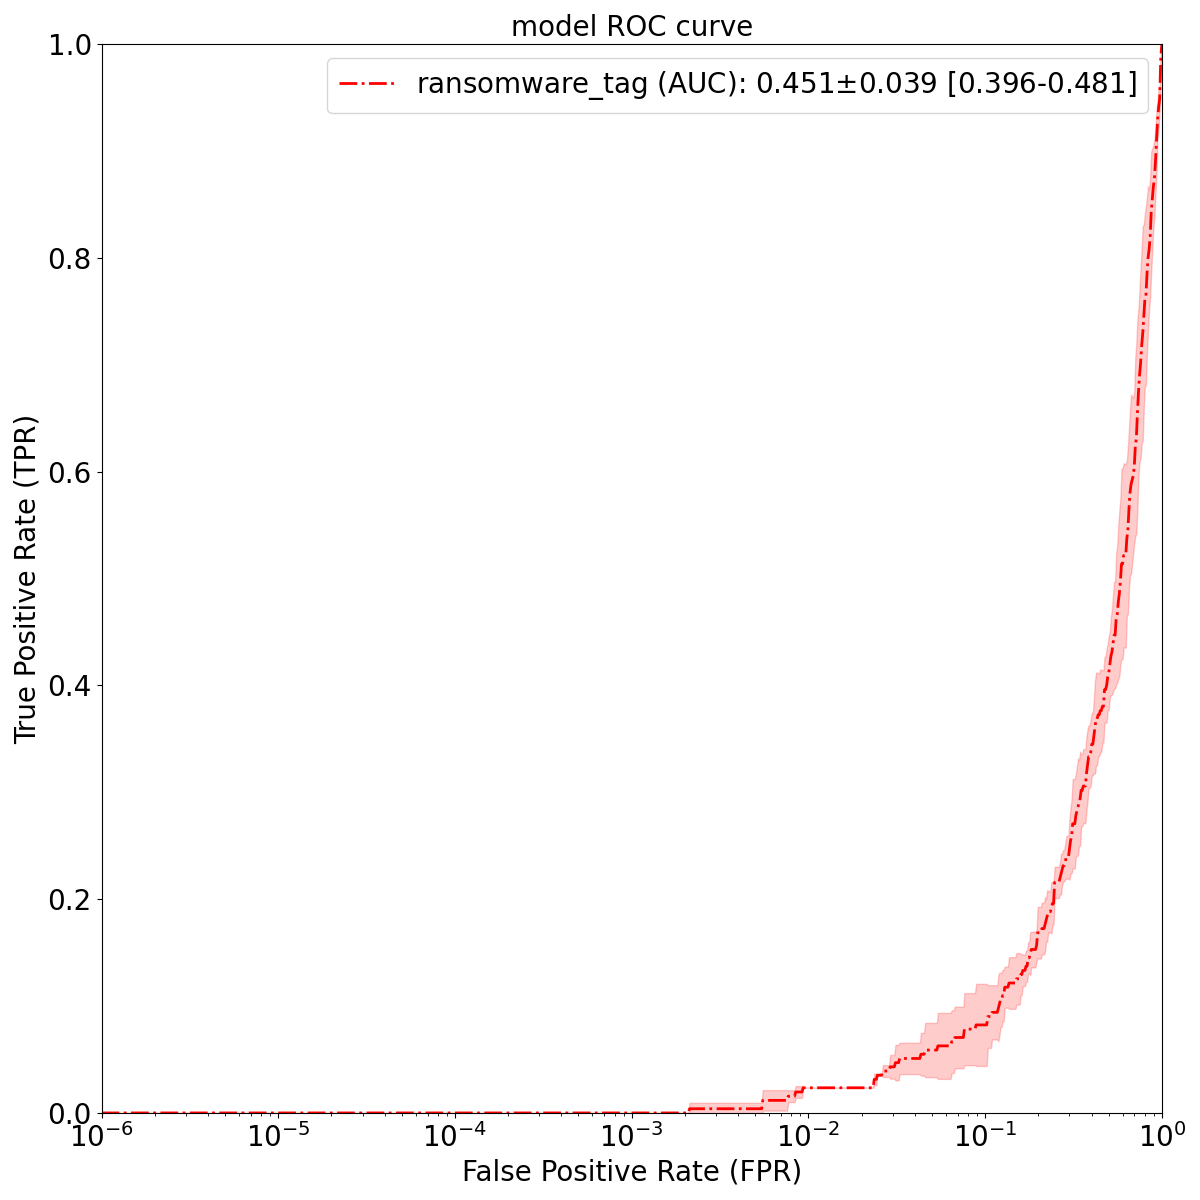
\includegraphics[width=0.6\textwidth]{./results/ransomware_tag_roc_aloha.png}
        \vspace*{-0.2cm}
        \caption{ROC curve and AUC statistics of \textBF{ALOHA} model for the \textbf{Ransomware Tag}. The line represents the \textit{mean} TPR at a given FPR, while the shaded region represents the \textit{standard deviation}. Statistics were computed over \textBF{3} training runs, each with random parameter initialization.}
        \label{fig:ransomwareTagRocAloha}
    \end{figure}
}

\newcommand{\ransomwareTagRocJointEmbedding}{
    \begin{figure}[H]
        \vspace*{-0.5cm}
        \centering
        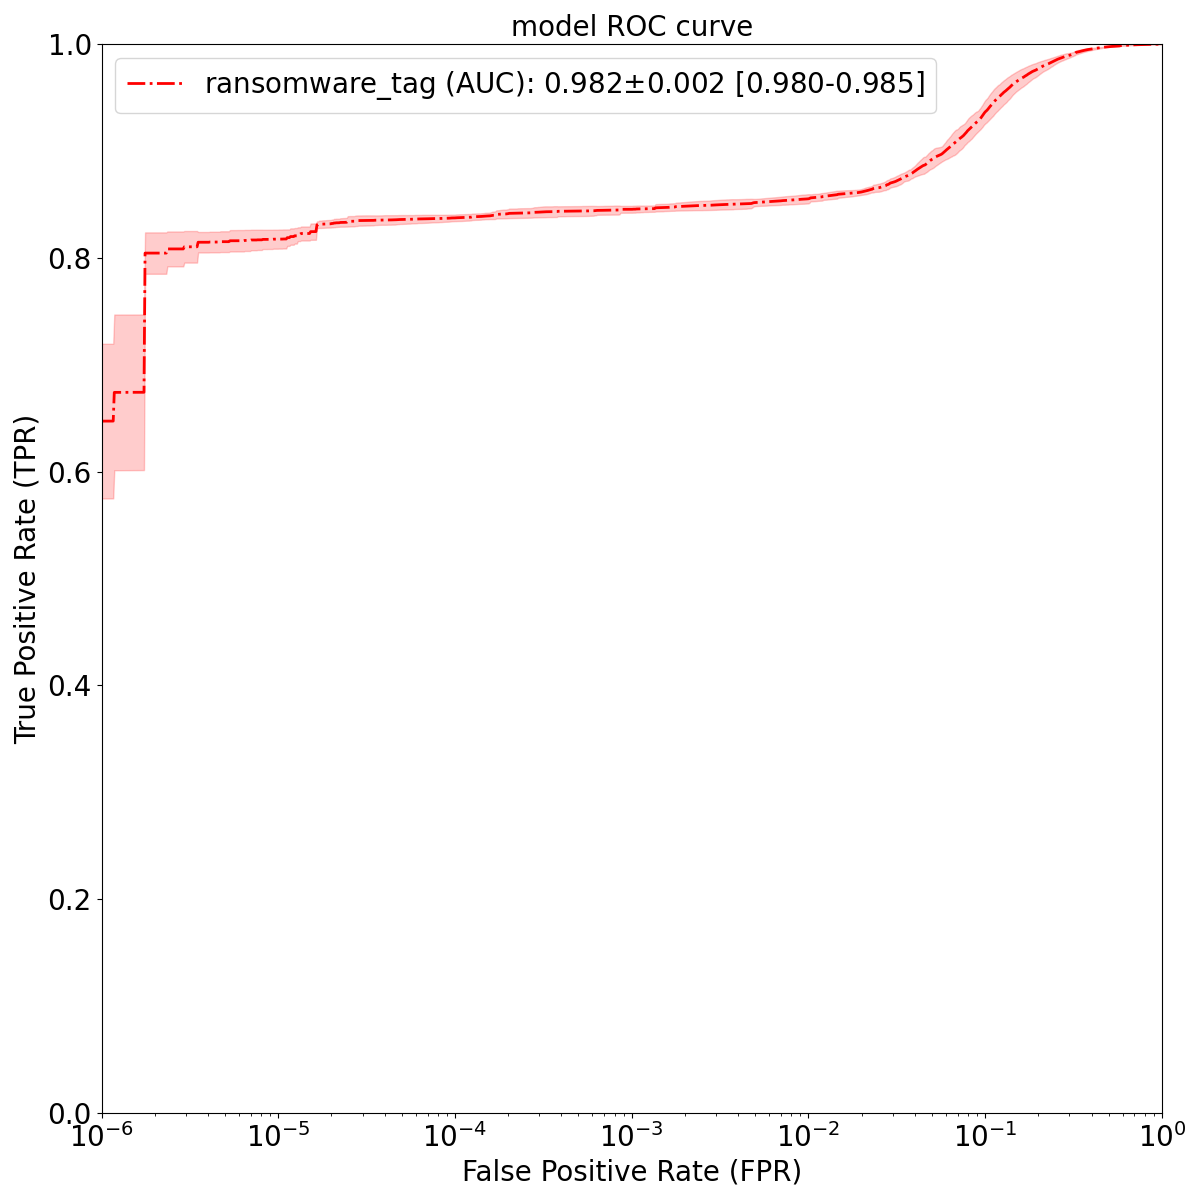
\includegraphics[width=0.6\textwidth]{./results/ransomware_tag_roc_jointEmbedding.png}
        \vspace*{-0.2cm}
        \caption{ROC curve and AUC statistics of \textBF{Joint Embedding} model for the \textbf{Ransomware Tag}. The line represents the \textit{mean} TPR at a given FPR, while the shaded region represents the \textit{standard deviation}. Statistics were computed over \textBF{3} training runs, each with random parameter initialization.}
        \label{fig:ransomwareTagRocJointEmbedding}
    \end{figure}
}

\newcommand{\ransomwareTagRocProposedMethod}{
    \begin{figure}[H]
        \vspace*{-0.5cm}
        \centering
        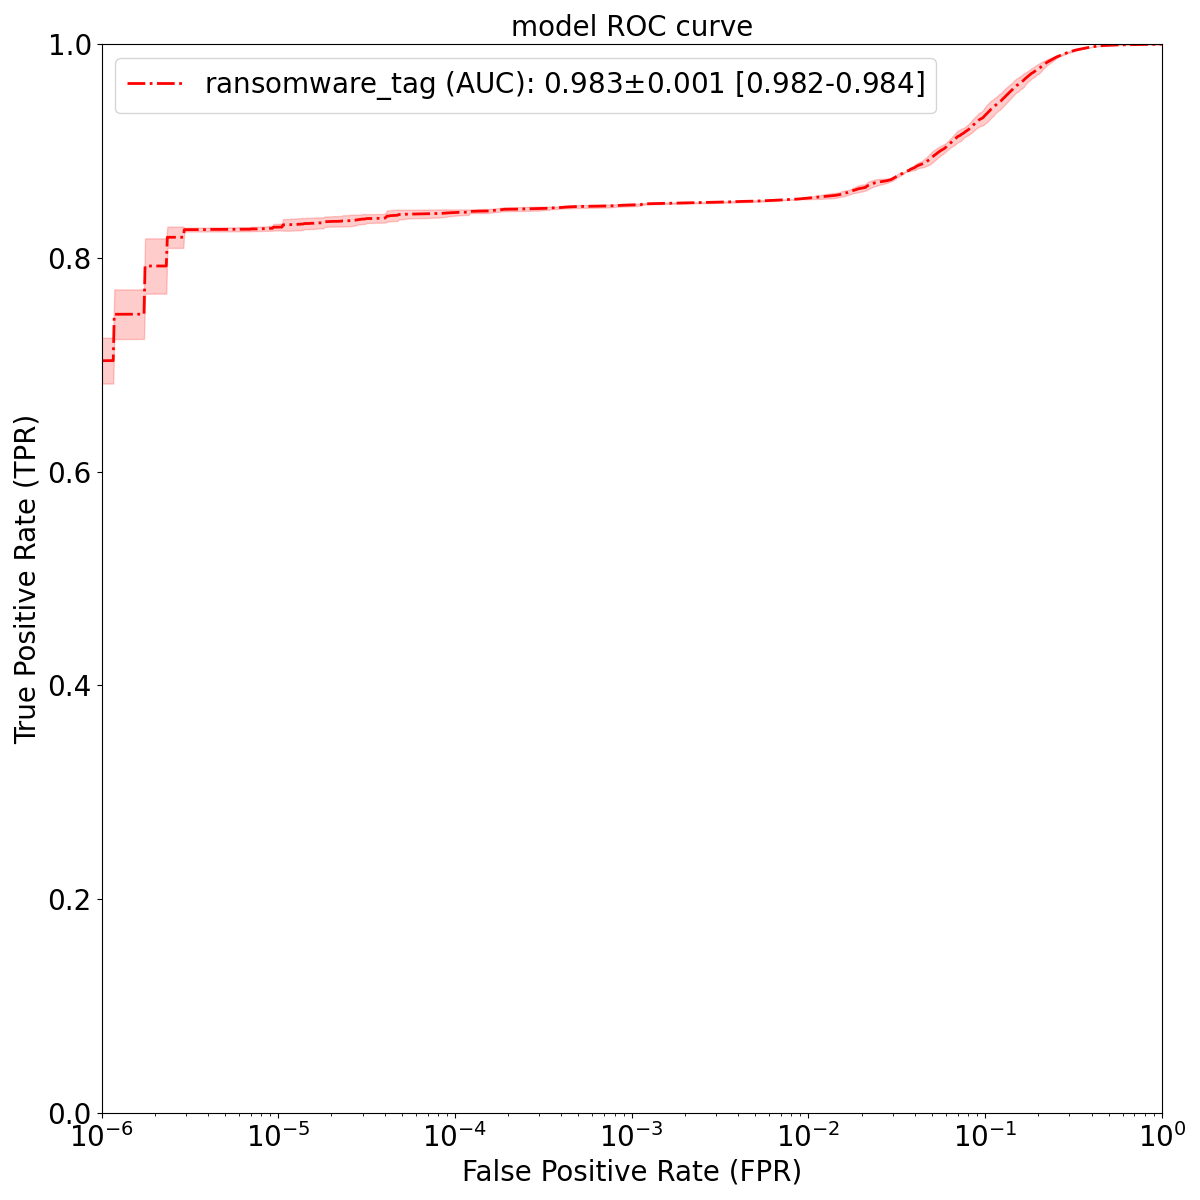
\includegraphics[width=0.6\textwidth]{./results/ransomware_tag_roc_proposedModel.png}
        \vspace*{-0.2cm}
        \caption{ROC curve and AUC statistics of \textBF{Proposed Model} for the \textbf{Ransomware Tag}. The line represents the \textit{mean} TPR at a given FPR, while the shaded region represents the \textit{standard deviation}. Statistics were computed over \textBF{3} training runs, each with random parameter initialization.}
        \label{fig:ransomwareTagRocProposedModel}
    \end{figure}
}
